\documentclass[tikz]{standalone}

\usepackage{tikz}
\usepackage{xcolor}
\usetikzlibrary{positioning, fit, backgrounds}

% Gentle, low-saturation colors, chosen to remain distinguishable when printed in grayscale
\definecolor{validfill}{RGB}{209,223,235}
\definecolor{validfill2}{RGB}{233,241,247}
\definecolor{validline}{RGB}{68,98,128}
\definecolor{relfill}{RGB}{224,190,152}
\definecolor{relfill2}{RGB}{241,222,199}
\definecolor{relline}{RGB}{150,98,58}
\definecolor{facciatafill}{RGB}{240,240,240}
\definecolor{facciataline}{RGB}{130,130,130}

\begin{document}

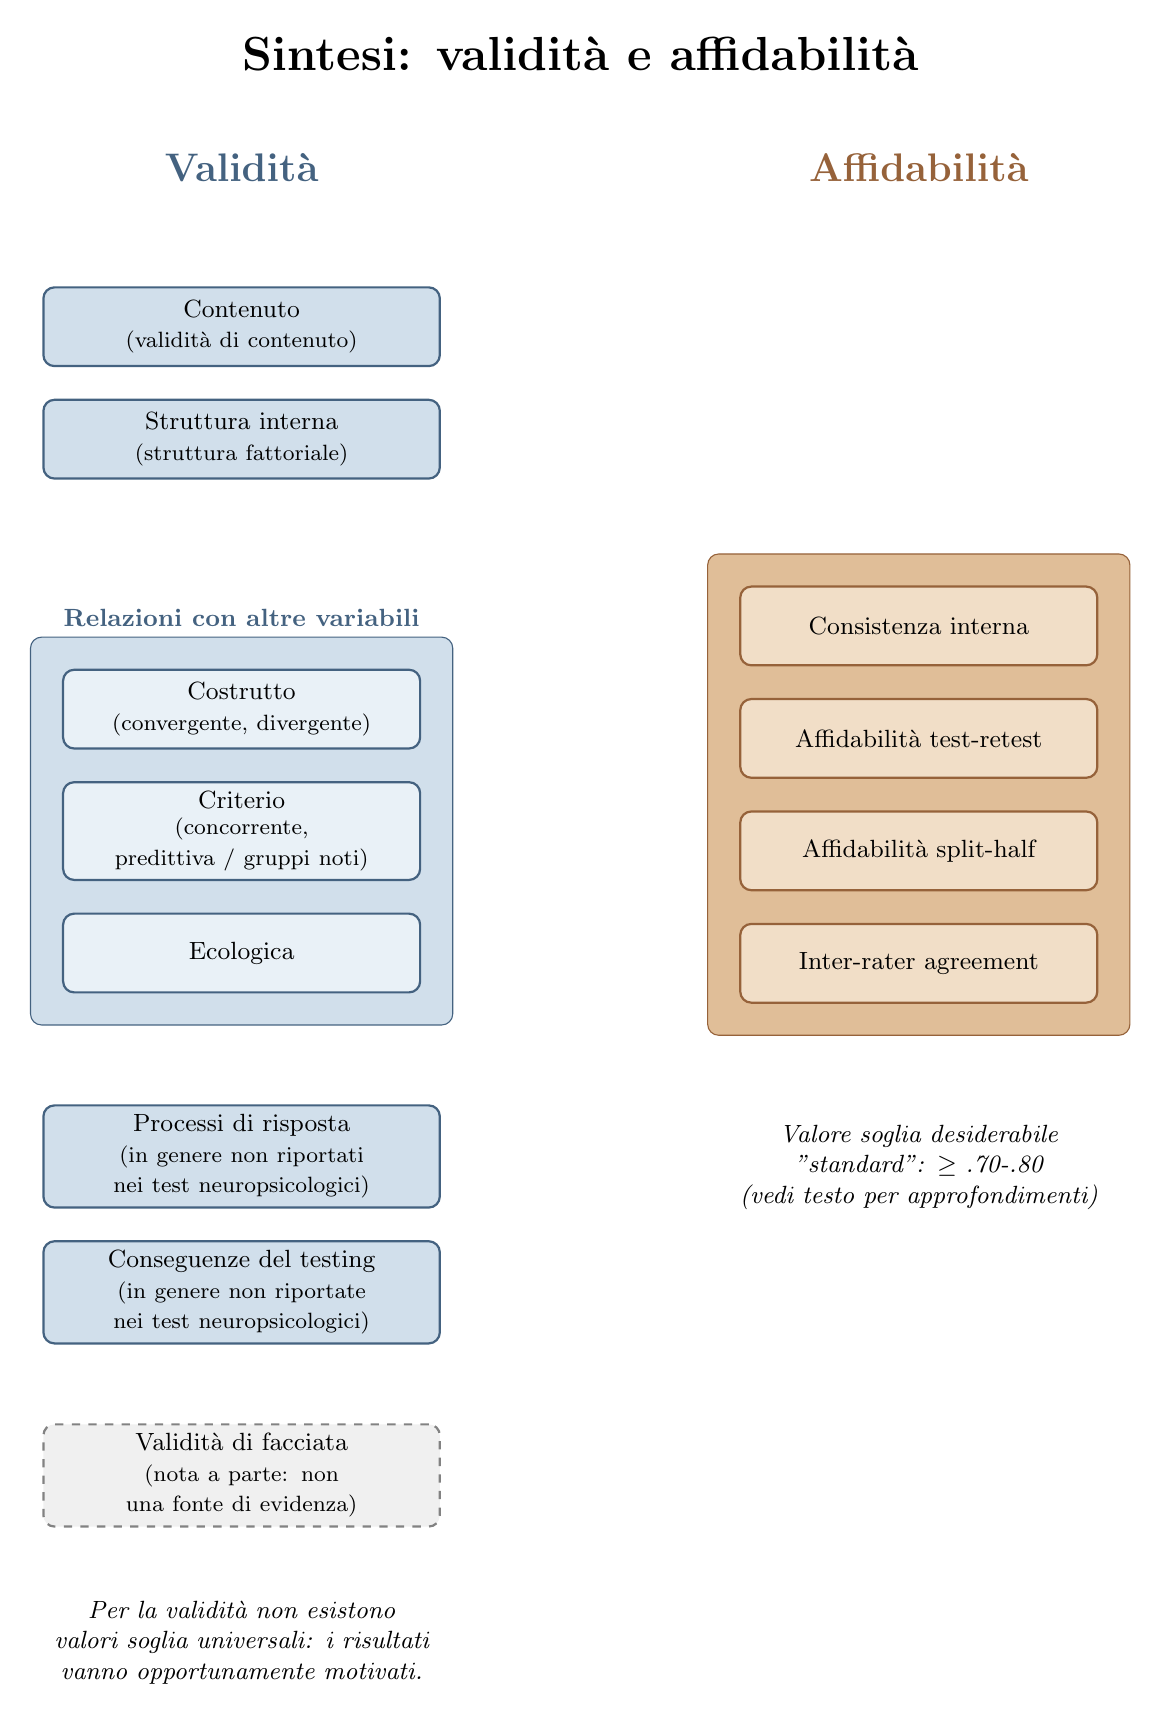
\begin{tikzpicture}[
    thick,
    box/.style={draw, rounded corners, align=center, text width=4.8cm, minimum height=1cm, font=\small},
    boxvalid/.style={box, fill=validfill, draw=validline},
    boxvalid2/.style={box, fill=validfill2, draw=validline, text width=4.3cm},
    boxrel/.style={box, fill=relfill, draw=relline},
    boxrel2/.style={box, fill=relfill2, draw=relline, text width=4.3cm},
    boxfacciata/.style={box, fill=facciatafill, draw=facciataline, dashed},
    colhead/.style={font=\bfseries\Large},
    note/.style={align=center, font=\small\itshape, text width=5.2cm}
]

% ---------- Title ----------
\node[font=\bfseries\LARGE] (title) at (0,0) {Sintesi: validità e affidabilità};

% ---------- Column headings ----------
\node[colhead, text=validline, below=8mm of title, xshift=-4.3cm] (validhead) {Validità};
\node[colhead, text=relline, below=8mm of title, xshift=4.3cm] (affhead) {Affidabilità};

% ---------- LEFT COLUMN: Validità (fonti di evidenza, Standards 2014) ----------
\node[boxvalid, below=12mm of validhead] (contenuto) {Contenuto \\ \footnotesize (validità di contenuto)};
\node[boxvalid, below=4mm of contenuto] (struttura) {Struttura interna \\ \footnotesize (struttura fattoriale)};

\node[boxvalid2, below=24mm of struttura] (costrutto) {Costrutto \\ \footnotesize (convergente, divergente)};
\node[boxvalid2, below=4mm of costrutto] (criterio) {Criterio \\ \footnotesize (concorrente, \\ predittiva / gruppi noti)};
\node[boxvalid2, below=4mm of criterio] (ecologica) {Ecologica};

\begin{scope}[on background layer]
\node[draw=validline, rounded corners, fill=validfill, fit=(costrutto)(criterio)(ecologica), inner sep=4mm, label={[font=\bfseries\small, text=validline]above:Relazioni con altre variabili}] (relbox) {};
\end{scope}

\node[boxvalid, below=10mm of relbox] (processi) {Processi di risposta \\ \footnotesize (in genere non riportati nei test neuropsicologici)};
\node[boxvalid, below=4mm of processi] (conseguenze) {Conseguenze del testing \\ \footnotesize (in genere non riportate nei test neuropsicologici)};

\node[boxfacciata, below=10mm of conseguenze] (facciata) {Validità di facciata \\ \footnotesize (nota a parte: non una fonte di evidenza)};

\node[note, below=8mm of facciata] (validnote) {Per la validità non esistono valori soglia universali: i risultati vanno opportunamente motivati.};

% ---------- RIGHT COLUMN: Affidabilità ----------
\node[boxrel2, below=50mm of affhead] (consistenza) {Consistenza interna};
\node[boxrel2, below=4mm of consistenza] (testretest) {Affidabilità test-retest};
\node[boxrel2, below=4mm of testretest] (splithalf) {Affidabilità split-half};
\node[boxrel2, below=4mm of splithalf] (interrater) {Inter-rater agreement};

\begin{scope}[on background layer]
\node[draw=relline, rounded corners, fill=relfill, fit=(consistenza)(testretest)(splithalf)(interrater), inner sep=4mm] (affbox) {};
\end{scope}

\node[note, below=10mm of affbox] (affnote) {Valore soglia desiderabile "standard": $\geq$ .70-.80 \\ (vedi testo per approfondimenti)};

\end{tikzpicture}

\end{document}
